%Bene
\newpage
\usecase{Wiederherstellung der Logindaten}
Der Nutzer hat nach einer gewissen Zeit seine Logindaten vergessen. Nun möchte er nach dem Abrufen der Seite versuchen seine Logindaten wiederherzustellen.

\usecasepart{Suchen des Wiederherstellungsformulars}

\problem{\enquote{Logindaten vergessen} an unüblicher Position}{
Der üblicherweise erste Schritt beim Wiederherstellen der Logindaten ist die Suche nach dem Login-Bereich. Erfahrungsgemäß befindet sich dort eine Weiterleitung mit der Möglichkeit das Passwort wiederherzustellen. Ein Nutzer, der diese Funktion auf der Webseite des Alumni-Portals nutzen möchte, findet keinen solchen Hinweis im blau hinterlegten Login-Bereich (siehe Abbildung \ref{fig:Wiederherstellung_1}). Erst beim zweiten oder dritten Blick, je nachdem welche Navigationsleiste der Nutzer zuerst durchsucht, stößt er auf den Hinweis \glqq Logindaten vergessen \grqq . Bereits diese Tatsache wirkt abschreckend auf den Nutzer und beeinträchtigt den Arbeitsfluss.
}{
Erfahrungsgemäß ist das Wiederherstellen der Logindaten zeitaufwändig. Wird ein Nutzer bereits beim Finden dieser Funktion auf der Webseite behindert, kann es schnell zur Frustration kommen (Kategorie 3).
}{
Die Option der Logindatenwiederherstellung gehört definitiv zum Bereich der Anmeldung auf einer Webseite. Aus diesem Grund ist diese Option üblicherweise auch im direkten, meist abgegrenzten Bereich, des Anmeldeformulars zu finden. Das Anmelden, Registrieren und die Passwortwiederherstellung fallen unter dieselbe Funktionsdomäne und sollten aus diesem Grund gemeinsam an einer Stelle gruppiert werden.
%\footnote{TODO:HCI 3rd Edition Page:132}
}

%#########################################################################
\usecasepart{Ausfüllen des Wiederherstellungsformulars}

\begin{figure}
	\centering
		
\includegraphics[width=\textwidth]{figures/Wiederherstellung_1.jpg}
		\caption{Wiederherstellungsformular für die Logindaten}
	\label{fig:Wiederherstellung_1}
\end{figure}

\subsubsection*{Positive Beobachtungen}
Der Bereich zum Wiederherstellen der Logindaten ist überschaubar gehalten. In zwei kurzen Textabschnitten wird dem Nutzer erklärt wie der Vorgang abläuft und was er dabei zu machen hat. Das Formular hat nur ein einziges Eingabefeld und wirkt aufgeräumt. Der Nutzer hat nicht viel Spielraum für falsche Interpretationen.%Das einzelne Eingabefeld zusammen mit der Beschreibung lässt somit keinen Spielraum für Fehlinterpretationen, auch bei potentiell unerfahrenen Nutzern. 

\problem{Text über den Rand hinaus geschrieben}{
Die Beschreibung zur Logindatenwiederherstellung wird über die Webseitenabgrenzung hinaus weiter geführt (siehe Abbildung \ref{fig:Wiederherstellung_1}). Die fehlende Formatierung des Textes wirkt unsauber und unprofessionell.
}{
Probleme solcher Art stören nicht direkt die Nutzung der Webseite, haben aber einen anderen negativen Effekt. Es stellt beim Nutzer die Seriosität des Portals in Frage, vor allem wenn an anderer Stelle nach vertraulichen Daten, beispielsweise der Bankverbindung, gefragt wird. Das ganze Auftreten des Alumni-Portals wird durch solche Formatierungsfehler in ein schlechtes Licht gerückt (Kategorie 1).
}{
Bei der Gestaltung von Texten sollte mehr Wert auf die Formatierung gelegt werden. Bestimmte Bereiche, in denen Text stehen kann, müssen unbedingt auch eingehalten werden.
}
\problem{Formularfeld nicht beschrieben}{
Das Formularfeld für die E-Mail-Adresse hat weder eine Beschreibung oberhalb, noch einen Platzhalter innerhalb des Feldes (siehe Abbildung \ref{fig:Wiederherstellung_1}). Es geht nur aus dem Text hervor welche Eingabe hier vom Nutzer verlangt wird.
}{
Die beiden beschreibenden Texte zur Logindatenwiederherstellung erklären zwar den Nutzen des Inputfeldes, auf den ersten Blick wird dieser allerdings nicht ersichtlich. Warum im Vergleich zum Registrierungsformular an dieser Stelle die Beschreibung entfernt wurde, ist fraglich. Für den Nutzer ist somit auf den ersten Blick unklar ob hier eine E-Mail-Adresse, der Benutzername oder eine gänzlich andere Information verlangt wird (Kategorie 1).
}{
Das Formularfeld sollte um eine passende Beschreibung ergänzt werden, entweder mit einem Textfeld darüber oder als Platzhalter innerhalb.
}
\problem{\glqq Senden \grqq ~Button mit Diskettensymbol}{
Der Button zum Absenden des Wiederherstellungsformulars enthält ein Diskettensymbol (siehe Abbildung \ref{fig:Wiederherstellung_1}). 
}{
Üblicherweise wird das Diskettensymbol bei Programmen dazu genutzt die gerade bearbeiteten Daten, meist beim Nutzer selbst, zu speichern. In dem Kontext dieser Webseite steht das Symbol für das Speichern der vom Nutzer eingegebenen Daten in der Datenbank des Alumni-Portals. Die Symbolik könnte bei einem Nutzer, dem dieser Hintergrund nicht bekannt ist, für Verwirrung sorgen (Kategorie 1).
}{
Eine Beschriftung des Buttons, der die Funktion des Formulars knapp beschreibt, wäre hier angebracht. Beschriftungen, die beispielsweise \enquote{Neues Passwort anfordern} oder \enquote{Neue Logindaten anfordern} lauten, wären sinnvoller.
}
\problem{Option für \glqq E-Mail-Adresse erkennen \grqq}{
Die Webseite bietet zwar die Möglichkeit dem Nutzer Logindaten, also Benutzername und Passwort, zukommen zu lassen. Allerdings gibt es keine Option die zur Anmeldung verwendete E-Mail-Adresse erkennen zu lassen. Einige Webseiten bieten ihren Nutzern diesen Service an.
}{
Ein Ziel des Alumni Portals ist es mit Kommilitonen und Dozenten auch noch Jahre nach dem Abschluss in Kontakt bleiben zu können. Da sich in dieser Zeit auch einmal die E-Mail-Adresse ändern kann ist es sinnvoll einen solchen Service zu bieten, auch wenn es sich hierbei per se nicht um Problem handelt (Kategorie 0).
}{
Unter der Option \glqq Logindaten vergessen \grqq ~befindet sich ein zusätzliches Formular, welches es dem Nutzer ermöglicht eine E-Mail-Adresse zu einem Benutzernamen erkennen zu lassen. Dabei wird eine E-Mail an die mit dem Benutzernamen verknüpfte Adresse versendet.
}

\begin{figure}
	\centering
		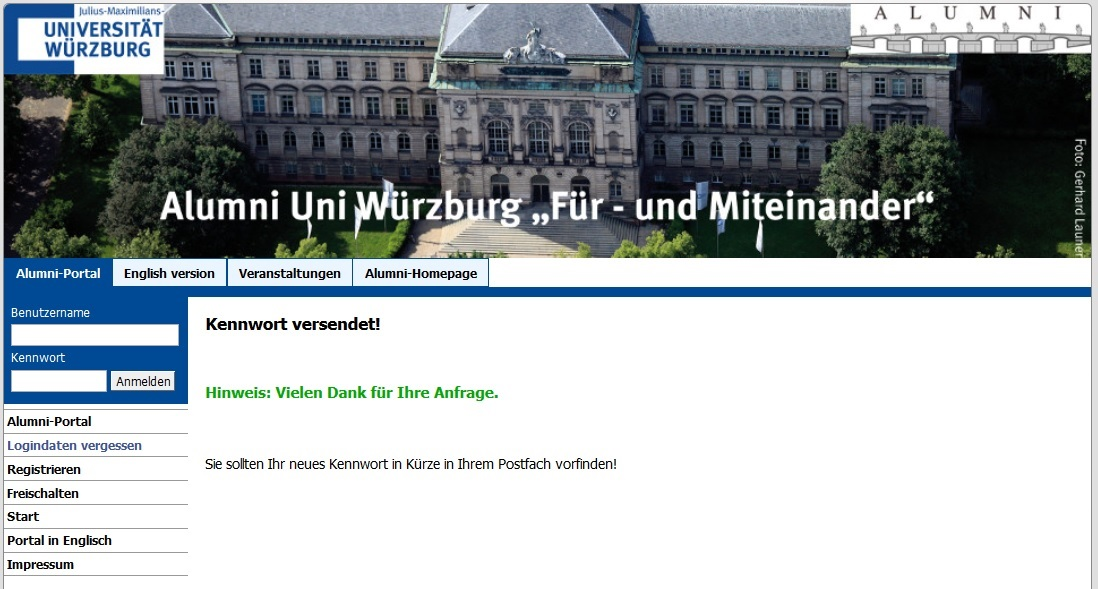
\includegraphics[width=\textwidth]{figures/Wiederherstellung_2.jpg}
		\caption{Feedback nach Absenden des Wiederherstellungsformulars}
	\label{fig:Wiederherstellung_2}
\end{figure}

\problem{Feedback-Meldung nicht konsistent mit anderen Meldungen}{
Nach dem Absenden des Formulars zur Wiederherstellung der Logindaten wird die gesamte Seite neu geladen. An Stelle des Absendeformulars erscheint eine fett gedruckte Benachrichtigung darüber, dass das Kennwort versendet wurde. Zusätzlich wird dem Nutzer mit einem grünen Text für seine Anfrage gedankt. In einer dritten Zeile wird in kleinerer Schriftgröße als in den anderen beiden Zeilen darauf hingewiesen, dass das neue Kennwort in Kürze im Postfach des Nutzers vorzufinden ist. In Abbildung \ref{fig:Wiederherstellung_2} sind diese drei unterschiedlichen Feedback-Nachrichten zu sehen.
}{
Feedback ist im Allgemeinen sehr wichtig für einen Nutzer, da er damit über den Status seiner Aktion mit dem System informiert werden kann. Im Fall der Passwortwiederherstellung erhält der Nutzer drei Nachrichten mit jeweils unterschiedlicher Darstellung des Textes. Darüber hinaus unterscheidet sich die Gestaltung anderer Feedback-Nachrichten der selben Webseite von Fall zu Fall. Das kann für Verwirrung beim Nutzer führen, da nicht ersichtlich ist, ob es einen Grund für die unterschiedlichen Darstellungen gibt (Kategorie 1).
}{
Positives sowie negatives Feedback vom System sollte konsistent sein, das heißt es soll die selbe Art und Weise einer Nutzerbenachrichtigung für die gesamte Webseite genutzt werden. Der Nutzer sollte unmissverständlich darüber in Kenntnis gesetzt werden, ob eine Interaktion mit der Webseite funktioniert hat und wenn nicht, worin der Fehler lag.
}

%#########################################################################
\usecasepart{Auslesen der Logindaten aus der E-Mail}
Das Formular wurde vom Nutzer ausgefüllt und abgesendet. Nun wartet der Nutzer auf die E-Mail mit den neu generierten Logindaten. 

\subsubsection*{Positive Beobachtungen}
Die E-Mail mit neuen Logindaten wird sehr schnell zugestellt. In der Regel war bereits beim Einloggen in den E-Mail-Account die Nachricht vorhanden.

\problem{Formale Anrede in E-Mail fehlt}{
Wurde das \glqq Logindaten vergessen \grqq ~Formular ausgefüllt, so erhält der Nutzer eine E-Mail mit den neu generierten Zugangsdaten. Bei dieser E-Mail fällt sofort auf, dass die gesamte Anrede fehlt. Die E-Mail beginnt, ohne jegliches Grußwort, mit \glqq Ihre Zugangsdaten lauten wie folgt: \grqq .
}{
Eine offizielle Webseite, wie in diesem Fall das Alumni-Portal, sollte mehr Wert auf die Umgangsform mit ihren Nutzern legen. Diese E-Mail verstärkt das Bild von Unprofessionalität und Unseriosität und ist einzustufen in der Kategorie der auffälligen Probleme (Kategorie 3).
}{
Die E-Mail sollte, passend zum Nutzer, eine persönliche, formale Anrede enthalten.
}
\problem{Fehlender Link zur direkten Anmeldung}{
In der E-Mail werden dem Nutzer die neu generierten Logindaten mitgeteilt. Ein Link, mit dem der Nutzer auf die Webseite geleitet, wird fehlt allerdings.
}{
Gewöhnlich befindet sich in einer E-Mail, mit der Userdaten oder Freischaltcodes versendet werde, ein Link, mit dessen Hilfe der Nutzer direkt auf die Webseite gelangt. Das verhindert einerseits den unnötigen Aufwand des Benutzers die Webseite manuell aufzurufen, andererseits können generierte Codes an den Link gehängt werden. Dabei würde gegebenenfalls das automatische Übertragen eines Freischaltcodes oder Passworts die Bedienung für den Nutzer erleichtern (Kategorie 2).
}{
Eine simple Verbesserung wäre ein Link mit dem ein Nutzer direkt zum Anmeldeformular kommt. Auch zu denken wäre eine Umsetzung, in der ein Nutzer direkt auf ein Formular zur Passwortänderung geleitet wird. Dort wird er dann aufgefordert, ein neues Passwort zu setzen.
}
%#########################################################################
\usecasepart{Anmelden mit neuen Logindaten}
Hat der Nutzer die E-Mail mit den neu generierten Logindaten erhalten, so ruft er die Webseite des Alumni-Portals auf, um sich damit das erste Mal einzuloggen. 

\subsubsection*{Positive Beobachtungen}
Das Anmelden mit den neuen Logindaten läuft ohne Probleme, es gibts nichts zu beanstanden.

%#########################################################################
\usecasepart{Setzen eines neuen Passworts}
Nach dem ersten Anmelden mit den neuen Logindaten wird ein Formular angezeigt, mit dem ein neues Kennwort gesetzt werden kann. 

\begin{figure}
	\centering
		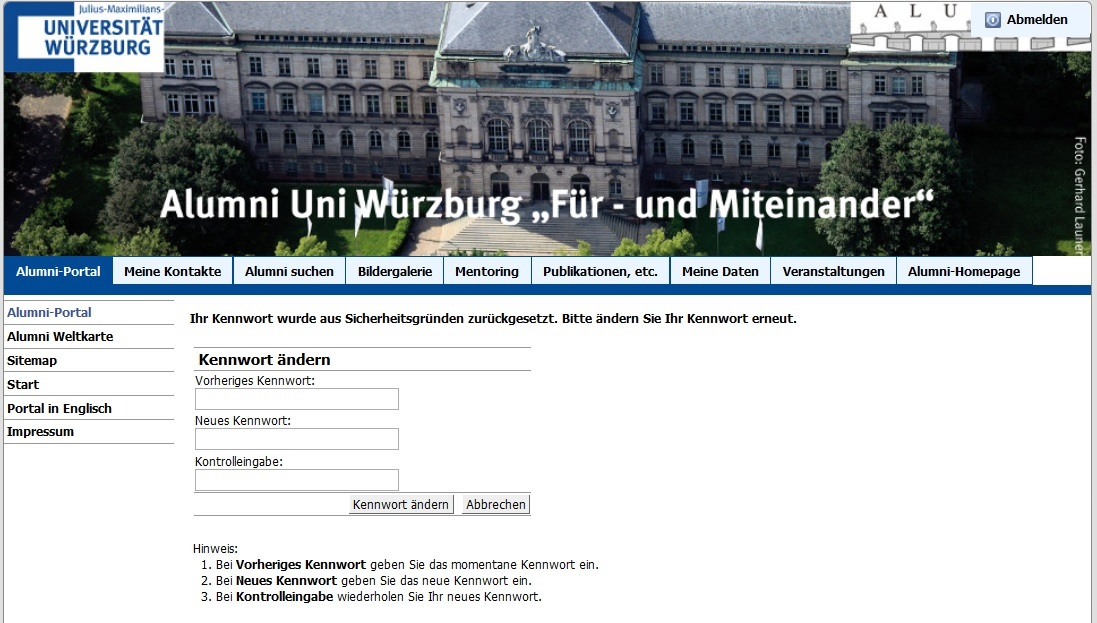
\includegraphics[width=\textwidth]{figures/Wiederherstellung_3.jpg}
		\caption{Formular zur Passwortänderung}
	\label{fig:Wiederherstellung_3}
\end{figure}

\subsubsection*{Positive Beobachtungen}
Die direkte Weiterleitung auf das Formular zum Ändern des Passwortes erleichtert dem Nutzer die Bedienung.

\problem{Fehlende Hinweise und Live-Validierung zu gültigen Passwörtern}{
Dem Formular zum Ändern des Passworts fehlt ein Hinweis darüber, welche Form ein Passwort haben muss oder darf. Es gibt weder einen Hinweis in Textform, noch gibt es irgendeine Art von Live-Validierung des Eingabefeldes (siehe Abbildung \ref{fig:Wiederherstellung_3}).}{
Ein Grund für das Wiederherstellen der Logindaten könnte darin bestehen, dass die Hinweise zu gültigen Kennwörtern bereits bei der Registrierung nicht ausreichend waren.\footnote{Beispiel: der fehlende Hinweis auf die Längenbegrenzung des Passworts auf 17 Zeichen.} Genau der selbe Fehler wird an dieser Stelle wiederholt. Bei dem Formular zur Änderung des Passworts steht kein Hinweis, wie eine gültige Passworteingabe auszusehen hat. Dieser Fakt ist äußerst ärgerlich für jeden Nutzer und mündet in Frustration. Ebenfalls wurde es versäumt eine Eingabevalidierung der Felder durchzuführen während das Passwort eingegeben wird bzw. wenn das Inputfeld verlassen wird. Lediglich beim Absenden des Formulars werden die Felder auf fehlerhafte Eingaben geprüft und der Nutzer darauf hingewiesen. Gerade bei Passwörtern ist das viel zu spät und damit nicht ausreichend. Störend und zugleich frustrierend ist dabei auch, dass die Eingabefelder nach dem erfolglosen Absenden geleert werden (Kategorie 4).
}{
Abhilfe würde ein einheitlicher Hinweistext schaffen, wann ein Passwort vom System akzeptiert wird und wann nicht. Ein solcher Hinweis könnte bei Eingaben des Nutzers leicht hervorgehoben werden, sobald dieser in das jeweilige Formularfeld klickt. Damit würde der Nutzer bei der Passwortwahl direkt darauf aufmerksam gemacht werden. Die fehlende Eingabevalidierung sollte ebenfalls implementiert werden. Durch kleine Hinweise kann der Nutzer direkt erkennen was er bei der Passwortwahl beachten muss oder vielleicht vergessen hat.}

\problem{Feedback bei der Passwortänderung}{
Das Feedback bei der Passwortänderung erscheint zwischen der oberen Navigationsleiste und dem Formular zur Passwortänderung. Der Einzeiler zur erfolgreichen Kennwortänderung entspricht wiederum nicht den anderen Feedbackmeldungen.
}{
Wie bereits bei den anderen Feedbackmeldungen bemängelt zeigt sich auch hier wieder eine Inkonsistenz zum Rest der Webseite (Kategorie 1).
}{
Ein mögliches Feedback sollte auch an dieser Stelle den Nutzer über die erfolgreiche Passwortänderung informieren. Eine solche Meldung sollte konsistent mit allen anderen Meldungen des Systems an den Nutzer sein. 
}
















